\chapter{Definición del problema}

\section{La comunicación corporativa}
La \emph{Comunicación Corporativa} se define como <<la totalidad de los recursos de comunicación de los que dispone una organización para llegar efectivamente a sus públicos>> \cite{riel_2001}. Dentro de este concepto, se distingue entre la \emph{Comunicación Corporativa Interna} y la \emph{Comunicación Corporativa Externa} siendo la primera <<todo lo relativo a la conexión requerida entre los miembros de una determinada estructura para acometer una metas comunes>> y la segunda, <<la vinculación de la organización con el entorno en el que desarrolla sus actividades, con el fin de alcanzar un determinado nivel de rentabilidad económica y social>> \cite{castro_2007}. Desde el ámbito empresarial y administrativo se da cada vez mayor importancia a la comunicación ya que ésta juega un papel fundamental en la consecución de sus objetivos.

Este tipo de comunicación ha encontrado en Internet uno de sus canales principales y tanto empresas como instituciones ejercen hoy en día su presencia online a través de webs, blogs, redes sociales o incluso sus propias aplicaciones para móviles, que han proliferado enormemente durante los últimos años \cite{playstore} \cite{appstore}. Todas estas herramientas permiten no sólo la publicación de comunicados sino también la planificación temporal, seguimiento y medida del impacto.

\section{Aplicaciones para móviles}
Aunque las redes sociales son uno de los medios preferidos por las empresas \cite{linkedin} y administraciones \cite{grande2015casos} como canal de comunicación debido a la gran acogida que tienen entre la población, las aplicaciones móviles son una alternativa muy a tener en cuenta ya que cubren la frecuente necesidad de incluir otros servicios específicos de la organización como por ejemplo:
\begin{itemize}
    \item Sistema de reservas (mesas en un restaurante, salas en un gimnasio\dots).
    \item Encuestas (toma de decisiones en una comunidad de vecinos, sondeo de la clientela de un bar para organizar un concierto en directo\dots)
    \item Sistema de geolocalización en tiempo real de un desfile (¿por dónde está pasando ahora mismo la cabalgata de reyes?).
\end{itemize}
Además, las aplicaciones salvan algunos de los inconvenientes de las redes sociales como la cesión de datos, la alta exposición a la crítica o la obligación de adaptarse al diseño y las reglas de negocio impuestas por un tercero.
También es necesario mencionar el enorme desarrollo que ha tenido el acceso a internet desde dispositivos móviles en los últimos años, como se puede observar en la figura \ref{fig:acceso-internet-tipo-dispositivo} \cite{dispositivos_internet_2019}.

\begin{figure}[ht]
    \centering
    % https://www.ontsi.red.es/es/indicadores/Hogares-y-ciudadanos/Internet/Dispositivos-de-acceso-Internet
    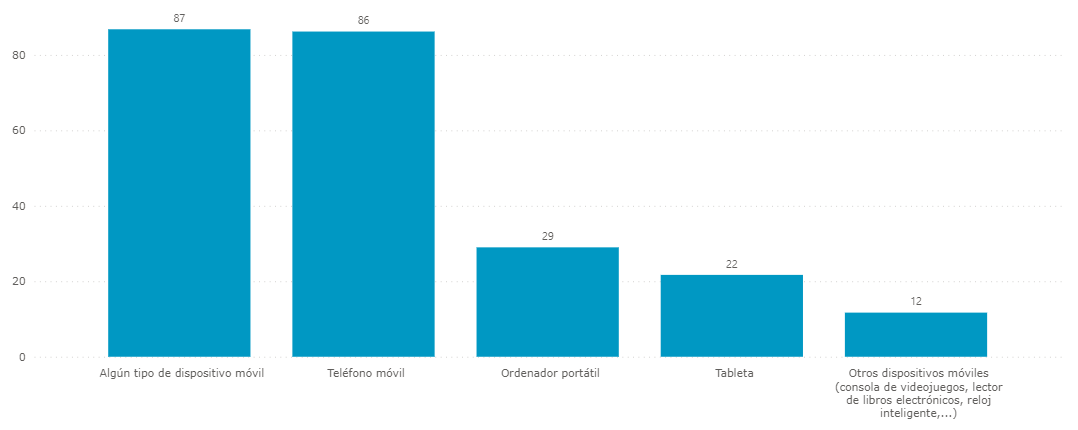
\includegraphics[scale=.5]{AccesoAInternetPorTipoDispositivo2019.png}
    \caption{Personas que han usado Internet en los últimos tres meses por tipo de dispositivo utilizado }
    \label{fig:acceso-internet-tipo-dispositivo}
\end{figure}